\documentclass[class=../../report, crop=false]{standalone}
\usepackage{graphicx}
\usepackage{float}

\begin{document}

\section{Final Prototype Details} \label{app:finaldetails}

\begin{table}[H]
	\centering
	\begin{tabular}{l | l | l}
		Specification & Target value & Final value \\ \hline
		Mass & 0.500kg & 0.350kg \\
		Top Speed & 2m/s & 1.56m/s \\
		Height & 87mm & 90mm \\
		Length & 152mm & 193mm \\
		Width & 77mm & 100mm \\
		Cost & \$100 & \$80.43 \\
		Batteries & 4 & 3 \\
	\end{tabular}
	\caption{Key Specifications for Target and Final Prototype}
	\label{app/table:targets}
\end{table}

\begin{figure}[H]
	\centering
	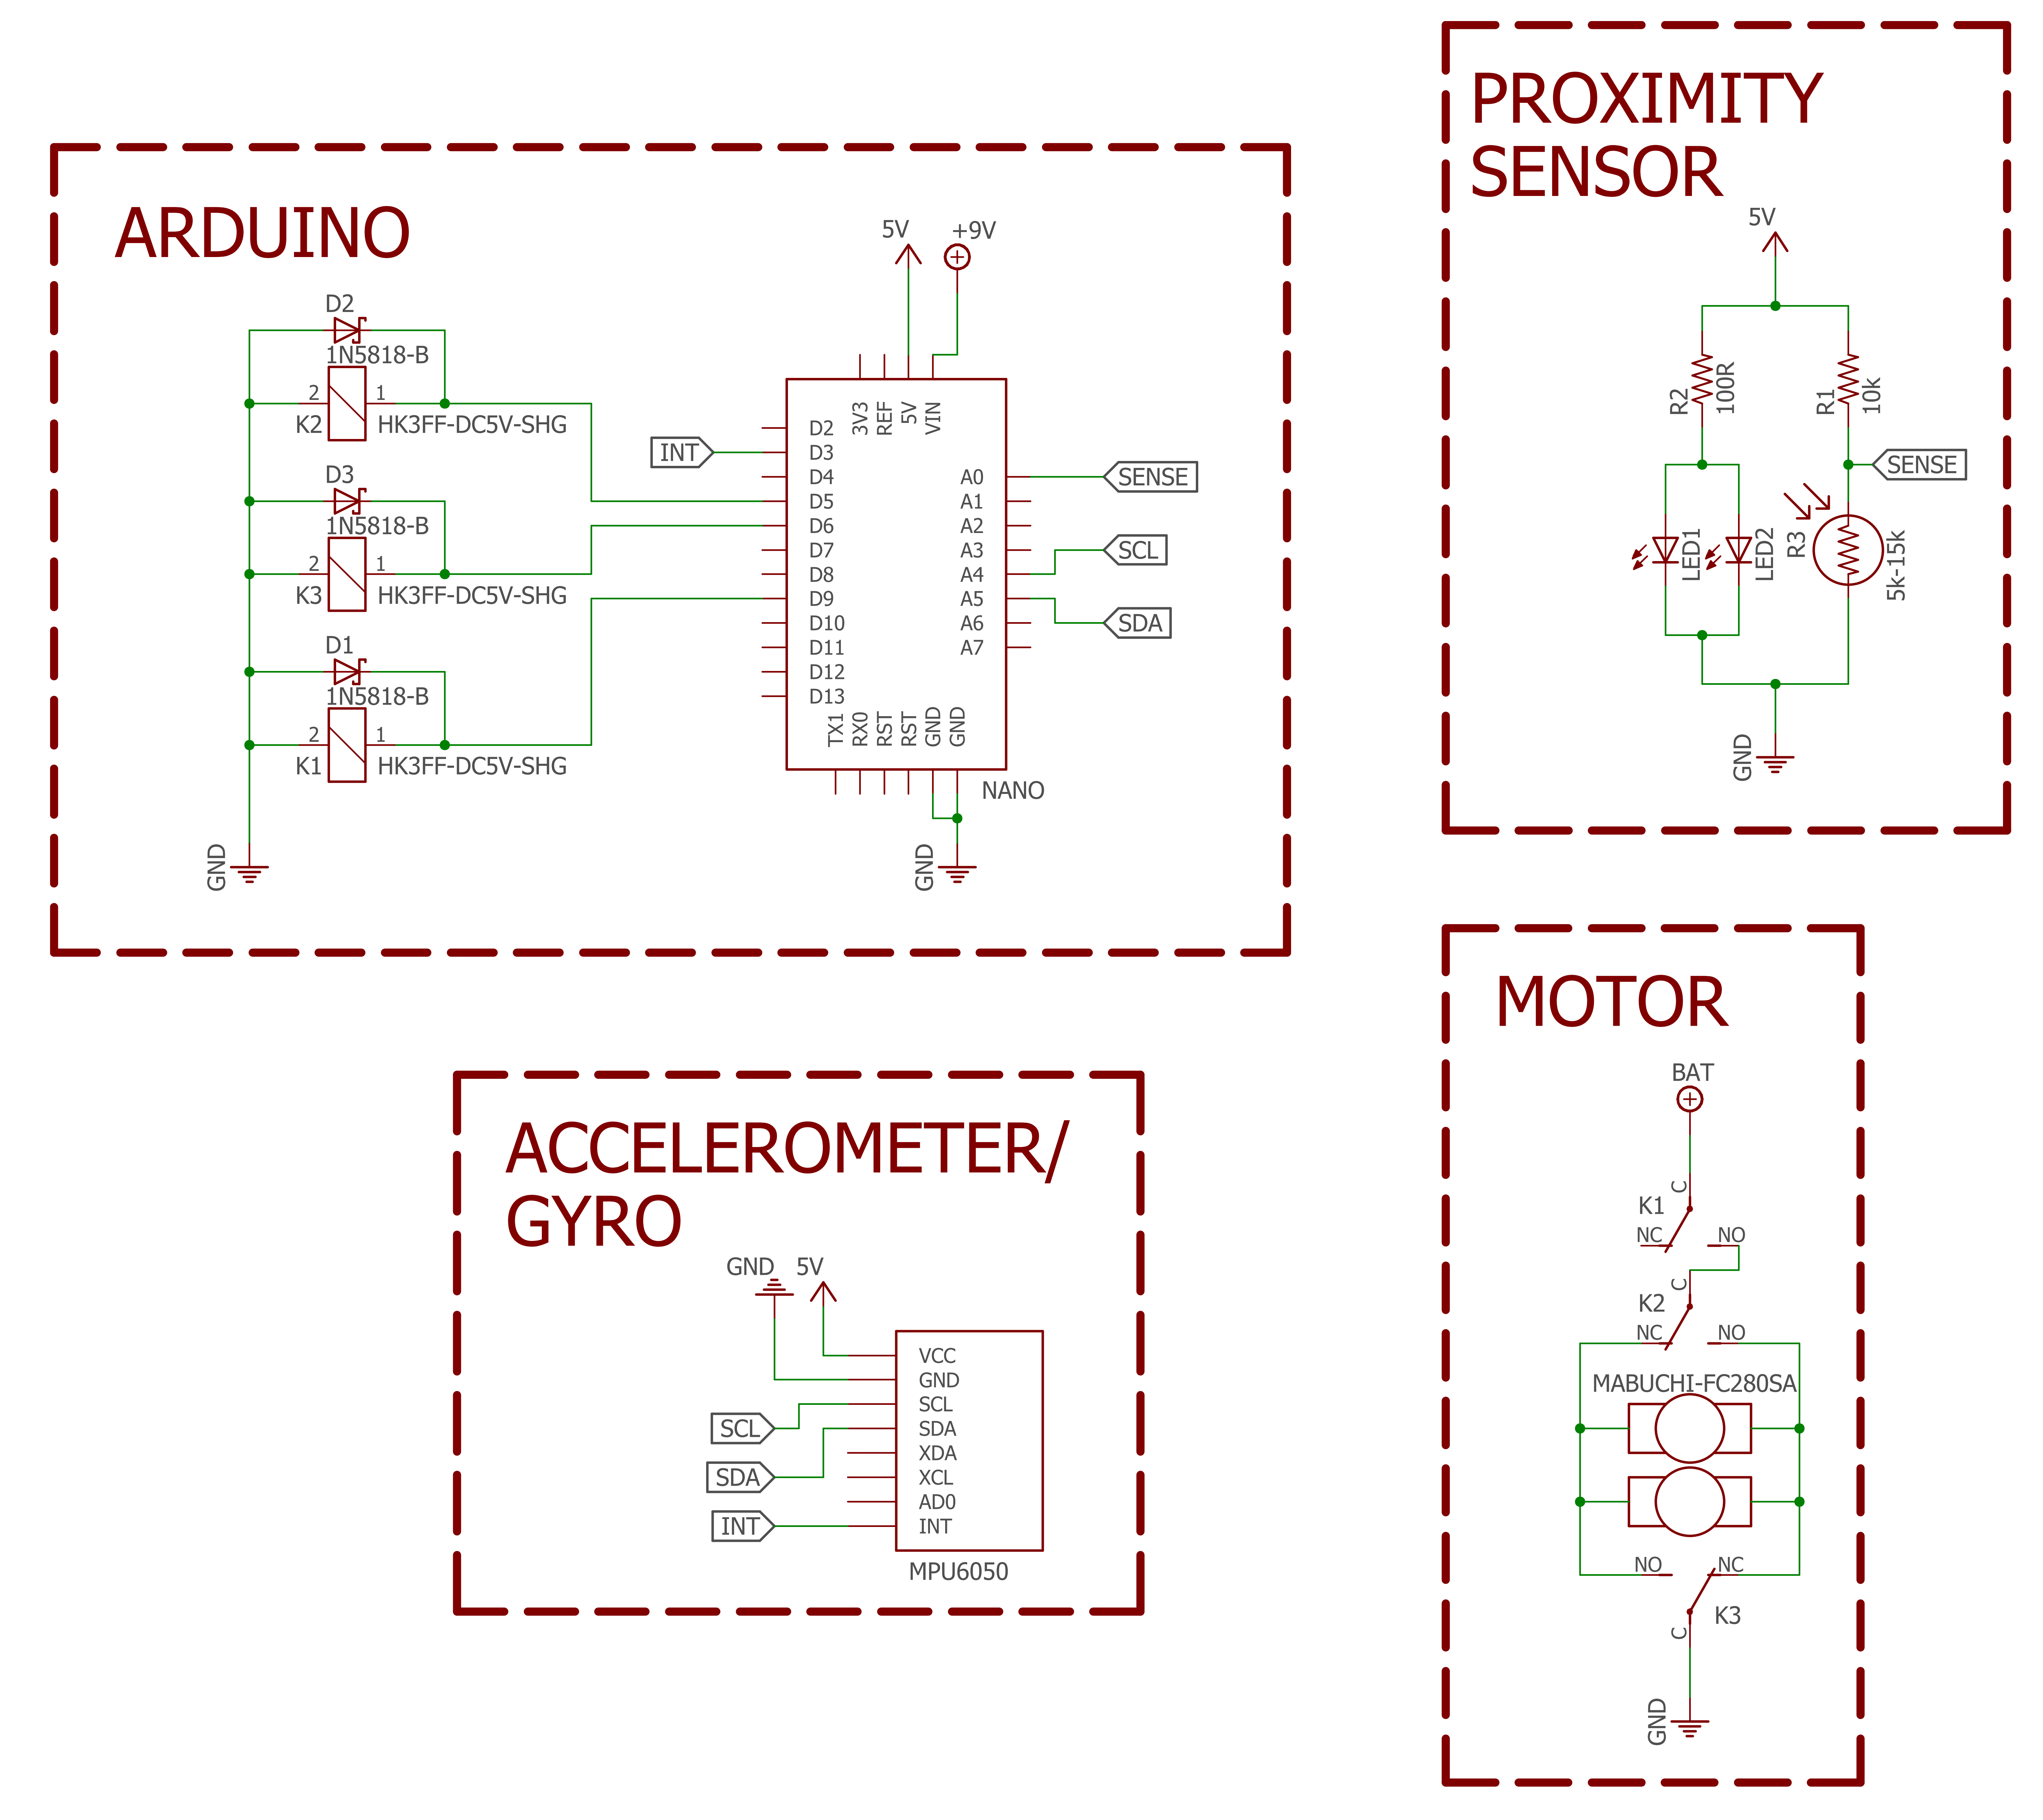
\includegraphics[width=0.8\textwidth]{../../res/img/circuit}
	\caption{Electrical System of Final Prototype}
	\label{app/fig:circuit}
\end{figure}

\begin{figure}[H]
	\centering
	\includegraphics[width=0.7\textwidth]{../../res/img/finalprototypecircuitry.png}
	\caption{Final Prototype Circuitry Mounts}
	\label{app/fig:finalprototypecircuitry}
\end{figure}

\end{document}
